\section{Brugergrænseflade}
\label{sec:webapplikationen}
Som resultat af prototypeafprøvningerne med informanter, som er beskrevet i afsnittene \ref{subsec:prototype1} og \ref{subsec:prototype2} følger her en præsentation og beskrivelse af den endelige brugergrænseflade. Vi har udviklet en webapplikation, som vi har valgt at kalde \Foodl{}.

Vi har valgt at gøre designet så enkelt som muligt for ikke at forvirre brugerne. Når man taster sig ind på hjemmesiden \url{http://www.foodl.dk}, bliver man mødt af en velkomsthilsen, der meget kort beskriver hjemmesidens formål og brug. Denne hilsen kan brugeren vælge at lukke ned. En cookie bliver gemt i browseren, så velkomsthilsnen ikke bliver vist igen, medmindre browserhistorikken bliver ryddet.

Figur \ref{fig:foodl-forside} viser forsiden af hjemmesiden, uden velkomsthilsnen. Navnet \Foodl{} er også en del af webapplikationens logo. For at gøre det mere klar for en ny bruger, hvad siden handler om, har vi erstattet et O i navnet med en stor ananas, fordi det er noget, der kan spises, og sidens formål er at give folk mulighed for at genbruge deres madrester. 

\begin{figure}[H]
	\centering
	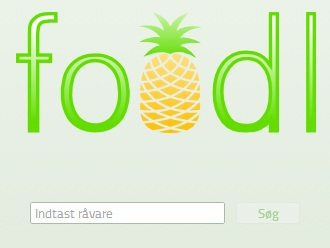
\includegraphics[scale=0.7]{billeder/foodl/forside.jpg}
	\capt{Denne figur viser webapplikationens startside.}
	\label{fig:foodl-forside}
\end{figure}

På alle undersider af \url{http://www.foodl.dk} er det muligt at tilgå sidehovedet. Her er der mulighed for at navigere tilbage til forsiden ved at klikke på den mindre version af det store logo, som blev vist på forsiden. Derudover kan man tilgå både en indkøbsliste og en liste af favorit-opskrifter, som brugeren selv vælger fra hjemmesiden. Både indkøbslisten og favoritter har et tal i parentes, der \fx fortæller brugeren, hvor mange varer, der er i den nuværende indkøbsliste eller hvor mange opskrifter, der er gemt under favoritter. Dette kan ses på \figref{fig:foodl-header}.

Ydermere kan man se på \figref{fig:foodl-header}, at det er muligt at logge ind eller oprette en bruger i webapplikationen. Dette er dog ikke obligatorisk, da vi ikke ønsker at binde brugerne til at oprette noget som helst. Man kan bruge systemet, om man har en bruger eller ej. Den eneste fordel ved at oprette en bruger er, at man på denne måde kan gemme indkøbslisten og favoritterne under hver bruger til fremtidigt brug.

\begin{figure}[H]
	\centering
	
\includegraphics[scale=0.7]{billeder/foodl/header.jpg}
	\capt{Denne figur viser webapplikationens sidehoved, hvilket kan ses på alle undersider.}
	\label{fig:foodl-header}
\end{figure}

Som sagt så har brugeren ikke behov for at logge ind for at bruge systemet. Det er nu op til brugeren at indtaste alle de råvarer, der ønskes brugt til madlavningen. Figur \ref{fig:foodl-soegefelt} viser, hvordan en sådan søgning foregår. Der bliver løbende indtastet bogstaver, og systemet undersøger for dele af tekststrenge, der matcher det der bliver indtastet. Ud fra disse match gives der forslag til hvilke råvarer, man kan vælge. Man kan ikke indtaste hvad som helst som et søgekriterie i systemet. Der er en lang række råvarer at vælge imellem. Hvis der \fx bliver indtastet kød i søgefeltet, så kommer der en liste af matchende råvarer som forslag, som man kan se på \figref{fig:foodl-soegefelt}.

For at fuldføre en søgning skal man blot trykke på ``Søg'', der er til højre for søgefeltet. Når brugeren trykker ``Søg'', så arbejder systemet på at finde alle de opskrifter, der minimum har en ingrediens, der matcher en af de indtastede råvarer.

\begin{figure}[H]
	\centering
	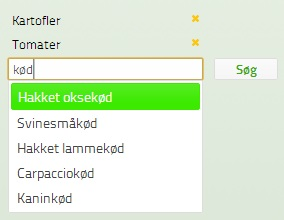
\includegraphics[scale=0.7]{billeder/foodl/soegefelt.jpg}
	\capt{Denne figur viser webapplikationens søgefelt.}
	\label{fig:foodl-soegefelt}
\end{figure}

Det er efter denne søgning, at brugeren finder ud af, hvad der er muligt at lave ud fra de råvarer, der er til rådighed. Resultatet er selvfølgelig afgrænset til den database man har over opskrifter.

Når søgningsresultatet vises, så er det en liste af opskrifter. I første omgang er opskrifterne sorteret efter relevans, dvs. hvor mange ingredienser, der matcher de forskellige indtastede råvarer. Figur \ref{fig:foodl-opskrift} viser et eksempel af en opskrift, der er et resultat af den foretagede søgning. I eksemplet er der kun 1 ingrediens, der matcher de indtastede råvarer, og denne er markeret med fed skrift (semidried tomatoes).

På hjemmesiden vises der kun hvilke ingredienser, der skal til for at lave opskriften, men selve fremgangsmåden er ikke vist nogen steder. Man er nødt til at tilgå den oprindelige hjemmeside, hvorfra opskriften stammer fra. Dette gøres ved at trykke på enten opskriftens titel eller billedet. Begge elementer består af et link til opskriftens originale hjemmeside. 

Fremgangsmåden kan ikke ses på vores hjemmeside, men alle andre vigtige elementer af opskriften er synlige. En opskrift består af følgende elementer:

\begin{itemize}[noitemsep]
\item Titel
\item Billede
\item Tilberedningstid
\item Relevans (antal matchende ingredienser)
\item Ingredienser
\item Knapper
\begin{itemize}[noitemsep]
\item Tilføj alle ingredienser til indkøbsliste
\item Tilføj / fjern fra favoritter
\item Tilføj enkelte ingredienser til indkøbsliste
\item Indmeld en fejl med opskriften
\end{itemize}
\end{itemize}

Alle opskrifter består af en beskrivende titel og et relevant billede, der skal vise brugeren, hvordan opskriften kan se. Billedet er med til at vække en interesse hos brugeren. Tilberedningstiden er også en vigtig ting at være klar over, og denne kommer direkte under billedet. De matchende ingredienser er markeret med fed skrift, så har brugeren nemmere ved at gennemskue, hvad der \fx er relevant at handle ind ud fra alle ingredienserne. Derudover er der et sæt knapper, som brugeren kan bruge. Se \figref{fig:foodl-opskrift}. I øverste højre hjørne er der en knap, der har et notesblok-lignende ikon. Denne knap tilføjer alle ingredienserne til indkøbslisten. Der er også mulighed for at tilføje de enkelte ingredienser ved at trykke på de små plus'er ud for ingredienserne. Ydermere er der mulighed for at tilføje og fjerne en opskrift til ens favorit-liste. Dette gøres ved at trykke på den hjerte-formede knap. I nederste højre hjørne er der en advarselsknap, der bruges til at rapportere om eventuelle fejl ved den specifikke opskrift.

\begin{figure}[H]
	\centering
	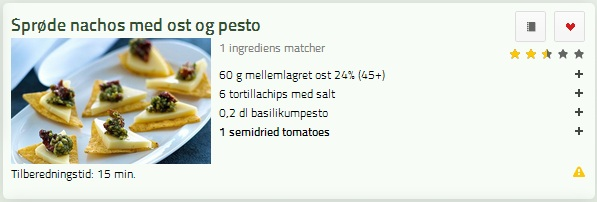
\includegraphics[scale=0.7]{billeder/foodl/opskrift.jpg}
	\capt{Her ses et eksempel på en opskrift, der kan være et resultat på en søgning.}
	\label{fig:foodl-opskrift}
\end{figure}

Brugeren har forskellige muligheder for at manipulere søgningsresultatet. Der er blevet implementeret en toolbar i toppen af siden, der følger brugerens bevægelser mht. at scrolle op og ned. På denne måde behøver brugeren ikke at scrolle helt til toppen for at udføre en handling på søgningsresultatet. 

Figur \ref{fig:foodl-toolbar} illustrerer, hvordan toolbaren ser ud. I venstre side er der en samling af tre knapper, der bruges til at begrænse søgningsresultatet mht. tilberedningstiden. Her er der mulighed for at markere flere af gangen, og default kriteriet er, hvis ingen er markeret, så er alle markeret. Dette betyder, at systemet starter med at vise alle resultater. I midten af toolbaren er der et skaleringsværktøj, der kan bruges til at skalere opskrifternes portioner mht. antal personer. Man kan skalere dem ned til 1 person og op til 10 personer. Vi valgte 10 som maximum, fordi det er relativt let at skalere yderligere, hvis dette er ønsket. Til højre er der endnu en samling af tre knapper, men disse benyttes til at sortere opskrifterne. Default er relevans. De to knappesamlinger er forskellige på to måder; hvad de bruges til, og at der kun er mulighed for at markere en knap af gangen ved sorteringsknapperne (højre side) og mulighed for markering af flere af gangen ved afgrænsningsknapperne (venstre side).

\begin{figure}[H]
	\centering
	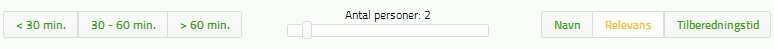
\includegraphics[scale=0.7]{billeder/foodl/toolbar.jpg}
	\capt{Webapplikationens toolbar, der er direkte under sidehovedet.}
	\label{fig:foodl-toolbar}
\end{figure}

Ud over toolbaren, så viser \figref{fig:foodl-sidebar} en sidebar, hvilket gør det mulight for brugeren at følge med i, hvad der bliver søgt på, og den er en mulighed for brugeren at lave endnu en søgning. Man kan herfra slette og/eller tilføje nye råvarer til en ny søgnign. Denne sidebar følger også brugeres scrolling, da det skal være nemt og hurtigt at lave en ny søgning, hvis dette bliver aktuelt.

\begin{figure}[H]
	\centering
	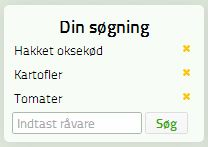
\includegraphics[scale=0.7]{billeder/foodl/sidebar.jpg}
	\capt{Webapplikationens sidebar, der vises ved resultatsiden.}
	\label{fig:foodl-sidebar}
\end{figure}

Hvis en bruger vælger at benytte sig af indkøbslisten, så kan denne tilgås via sidehovedet, som kan ses på \figref{fig:foodl-header}, ved at trykke på ``indkøbsliste''. I sidehovedet kan man også se, hvor mange varer, der er blevet tilføjet til listen. 

Man kan tilføje hvilken som helst tekststreng til indkøbslisten. På denne måde har vi ikke begrænset brugeren til blot at tilføje ingredienser fra opskrifterne, men det er helt op til brugeren selv at bestemme, hvad skal på listen. Brugeren har mulighed for at tilføje varer i feltet ``tilføj til indkøbsliste'' og trykke på ``tilføj''. Der er mulighed for at slette alle varer fra indkøbslisten og ligeledes at slette enkelte varer. Derudover er der implementeret en knap, til at udskrive indkøbslisten, hvis det skulle være nødvendigt.

\begin{figure}[H]
	\centering
	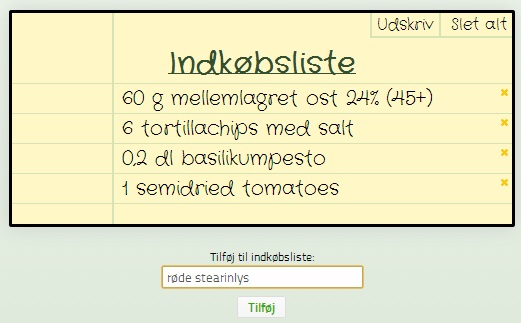
\includegraphics[scale=0.7]{billeder/foodl/indkoebsliste.jpg}
	\capt{Indkøbslisten tilgås fra sidehovedet.}
	\label{fig:foodl-indkoebsliste}
\end{figure}

I \figref{fig:foodl-opskrift} vises en knap, der bruges til at rapportere eventuelle fejl ved de specifikke opskrifter. Figur \ref{fig:foodl-fejlrapportering} viser, hvordan det ser ud, når en bruger trykker på rapporteringsknappen ved en opskrift. Der popper en lille boks op, og baggrunden af siden bliver mørk. Her kan man nu specificere, hvad fejlen handler om og give en beskrivelse, inden man vælger at indsende fejlen.

\begin{figure}[H]
	\centering
	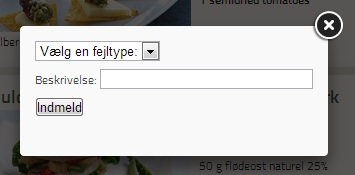
\includegraphics[scale=0.7]{billeder/foodl/fejlrapportering.jpg}
	\capt{Webapplikationens fejlraportering.}
	\label{fig:foodl-fejlrapportering}
\end{figure}

Muligheden for oprettelse af bruger er tilstede. Figur \ref{fig:foodl-opret} viser, hvordan denne ``log ind / opret bruger'' side ser ud. Man skal bruge sin email og en adgangskode for at lave en bruger. Hvis man allerede har en bruger, så skal man blot logge ind med de rigtige oplysninger. Som det tidligere blev nævnt, så er det ikke obligatorisk at oprette en bruger. Den eneste fordel der er ved dette er, at man får mulighed for at gemme indkøbslisten og listen over favoritter. 

Når man er logget ind, så ændrer sidehovedet sig en smule. Figur \ref{fig:foodl-loggetind} viser, at der nu er mulighed for at gå ind i en menu, der hedder ``indstillinger'' og at logge ud igen. Man kan også se, at der pludselig er indlæst en liste af favoritter på 10 opskrifter fra tidligere besøg.

\begin{figure}[H]
	\centering
	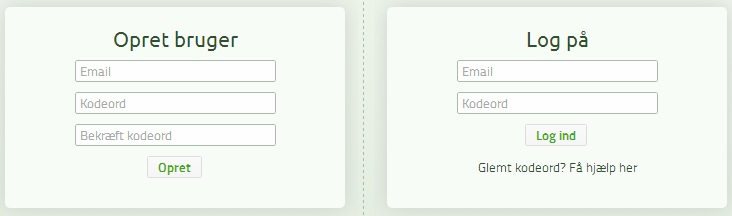
\includegraphics[scale=0.7]{billeder/foodl/login-opret.jpg}
	\capt{Webapplikationen giver brugeren mulighed for at oprette en bruger og logge ind med denne.}
	\label{fig:foodl-opret}
\end{figure}

\begin{figure}[H]
	\centering
	
\includegraphics[scale=0.7]{billeder/foodl/header-login.jpg}
	\capt{Det ændrede sidehovede, når brugeren er logget ind.}
	\label{fig:foodl-loggetind}
\end{figure}

Hvis man ønsker at skifte sin adgangskode, så sker det ved at trykke på knappen ``indstillinger'' i sidehovedet. Dette illustrerer \figref{fig:foodl-indstillinger}.

\begin{figure}[H]
	\centering
	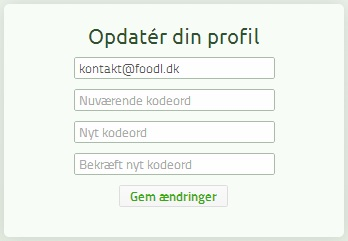
\includegraphics[scale=0.7]{billeder/foodl/indstillinger.jpg}
	\capt{Brugeren har mulighed for at ændre nogle basale indstillinger ved at klikke på ``indstillinger'' i sidehovedet.}
	\label{fig:foodl-indstillinger}
\end{figure}

Som de fleste andre hjemmesider, så har vi også en ``om'' og en ``kontakt'' side, som kan tilgås fra nederste venstre hjørne af enhver foodl-underside. Derudover kan man rapportere en generel fejl ved siden, hvis man støder på sådan en.

\begin{figure}[H]
	\centering
	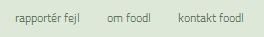
\includegraphics[scale=0.7]{billeder/foodl/formaliteter.jpg}
	\capt{I nederste venstre hjørne af webapplikationen kan man rapportere en generel fejl, læse mere om webapplikationen og kontakte udviklerne.}
	\label{fig:foodl-formaliteter}
\end{figure}
